\chapter{Diseño del sistema}
En este capítulo se realizará un análisis exhaustivo del software a desarrollar permitiendo bosquejar el resultado final de la aplicación, teniendo en cuenta los diferentes casos de uso. 

\section{Análisis de Requisitos}
Es fundamental definir una serie de requerimientos en el proyecto, ya que esto establece las bases y necesidades o expectativas que debe cumplir el sistema a desarrollar. En esta sección se analizarán dichos requerimientos comprendiendo las funcionalidades clave, expectativas de los usuarios y objetivos del proyecto.

\subsection{Requisitos funcionales}
\begin{enumerate}[label=RF\arabic*,leftmargin=2cm]
    \item Gestionar ingredientes. Esta funcionalidad permite gestionar los ingredientes de los que dispone el usuario.
    \begin{enumerate}[label=RF1.\arabic*] 
        \item Añadir. Esta funcionalidad permite añadir ingredientes a la despensa del usuario.
        \item Eliminar. Será posible eliminar ingredientes erróneos de la despensa. 
    \end{enumerate}
    \item Buscador de recetas. Esta funcionalidad permite al usuario encontrar recetas en la plataforma.
    \begin{enumerate}[label=RF2.\arabic*]
        \item Encontrar recetas en base a los ingredientes en la despensa. Debe ser posible encontrar recetas teniendo solo en cuenta los ingredientes que se encuentran actualmente en el inventario del usuario.
        \item Explorar todas las recetas. Será posible observar todas las recetas de las que dispone la aplicación.
        \begin{enumerate}[label=RF2.2.\arabic*]
            \item Filtrar por ingrediente. Esta funcionalidad permitirá filtrar recetas para observar aquellas que contengan un ingrediente concreto.
            \item Filtrar por tipo de cocina. Esta funcionalidad permitirá filtrar recetas por gastronomía. 
        \end{enumerate}
    \end{enumerate}
    \item Introducir restricciones alimentarias. Esta funcionalidad permitirá eliminar de manera automática las recetas con ingredientes conflictivos de la lista de resultados del buscador.
    \item Visualizar recetas. Se permitirá al usuario visualizar la receta del plato que el usuario quiere preparar.
\end{enumerate} 

\subsection{Requisitos no funcionales}
\begin{enumerate}[label=RNF\arabic*,leftmargin=2cm]
    \item Usabilidad. El software debe ser sencillo de usar, con una interfaz de usuario clara y organizada.
    \begin{enumerate}[label=RNF1.]
        \item Aprendizaje. El sistema debe tener una curva de aprendizaje menor a 2 horas. 
        \item Introducir ingrediente. Se deben poder introducir los ingredientes de manera sencilla. 
        \item Buscador. Es necesario que el buscador sea organizado y claro, para no entorpecer la búsqueda de recetas. 
        \item Visualizar recetas. La pantalla de recetas debe estar claramente organizada. Permitiendo que sea sencillo para el usuario ver los ingredientes y pasos a seguir. 
        \item Ajuste de letra. Se debe poder cambiar el tamaño de letra para ajustarse a las dificultades visuales de cada usuario.
    \end{enumerate}
    \item Mantenibilidad. El código debe estar correctamente estructurado y documentado para facilitar su mantenimiento en el tiempo.
    \begin{enumerate}[label=RNF2.\arabic*]
        \item Control de versiones. Será necesario utilizar una herramienta de control de versiones para llevar un seguimiento del proyecto y mejorar la calidad del producto final.
        \item Metodología. Será necesario seguir una correcta metodología para que el desarrollo del sistema sea lo más eficiente y simple posible.
    \end{enumerate}
    \item Compatibilidad. La aplicación debe ser compatible con el mayor número de dispositivos.
    \begin{enumerate}[label=RNF3.\arabic*]
        \item El sistema debe ser capaz de usarse desde diferentes plataformas para maximizar el número de usuarios.
    \end{enumerate}
    
    
\end{enumerate}

\section{Análisis funcional}
\subsection{Diagrama UML}
En esta sección se describe de manera sencilla el diagrama del software. Simplificando la implementación de la aplicación.

\begin{figure}[h!]
\centering
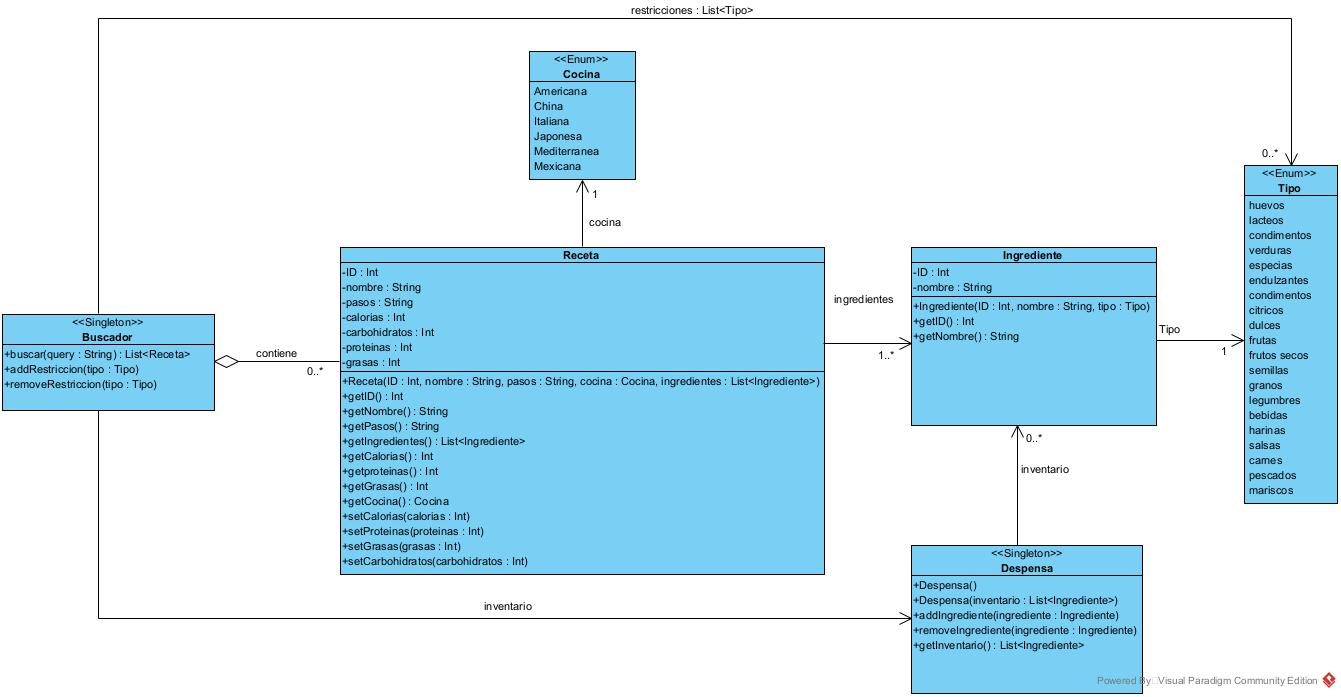
\includegraphics[width=125mm,scale=1]{imagenes/Class Diagram1.jpg}
\caption{Diagrama UML del proyecto}
\label{fig:UML}
\end{figure}

\subsection{Casos de uso}
Para representar correctamente las diferentes funcionalidades que cubran los requisitos expuestos anteriormente. Por ello se detallan los casos de uso de la aplicación.
\begin{table}[H]
\begin{tabular}{|m{3cm}|m{9cm}|}
\hline
\textbf{CU-01} & Introducir ingredientes en la despensa \\
\hline
\textbf{Descripción} & El sistema debe permitir introducir los ingredientes del usuario en la despensa, con el objetivo de limitar la búsqueda de recetas a aquellas que contengan los ingredientes con los que cuenta el usuario.\\
\hline
\textbf{Precondiciones} & Ninguna. \\
\hline
\textbf{Flujo Principal} & 
1. El usuario utiliza el buscador para encontrar el ingrediente. \\
& 2. Se asegura que es el ingrediente que quiere añadir. \\
& 3. Añade el ingrediente \\
\hline
\textbf{Excepciones} & El usuario busca un ingrediente no permitido. \\
\hline
\textbf{Postcondiciones} & El ingrediente queda añadido al inventario del usuario. \\
\hline
\end{tabular}
\label{Tab:Cu-01}
\end{table}
\begin{table}[H]
\begin{tabular}{|m{3cm}|m{9cm}|}
\hline
\textbf{CU-02} & Eliminar ingredientes en la despensa \\
\hline
\textbf{Descripción} & El sistema debe permitir eliminar los ingredientes que existan en el inventario del usuario.\\
\hline
\textbf{Precondiciones} & El ingrediente que se quiere eliminar debe estar en el inventario actual del usuario. \\
\hline
\textbf{Flujo Principal} & 
1. El usuario comprueba su despensa. \\
& 2. Elimina el ingrediente. \\
& 3. Acepta la eliminación del ingrediente. \\
\hline
\textbf{Excepciones} & El ingrediente no está en la despensa del usuario. \\
\hline
\textbf{Postcondiciones} & El ingrediente se borra del inventario del usuario.\\
\hline
\end{tabular}
\label{Tab:Cu-02}
\end{table}
\begin{table}[H]
\begin{tabular}{|m{3cm}|m{9cm}|}
\hline
\textbf{CU-03} & Añadir restricciones al buscador \\
\hline
\textbf{Descripción} & El sistema debe permitir añadir una serie de restricciones dietéticas al buscador, para usuarios que tengan una determinada dieta debido a alergias o intolerancias.\\
\hline
\textbf{Precondiciones} & Ninguna. \\
\hline
\textbf{Flujo Principal} & 
1. El usuario añade la restricción al buscador. \\
\hline
\textbf{Excepciones} & No existe el tipo de ingrediente introducido. \\
\hline
\textbf{Postcondiciones} & La restricción queda reflejada en el buscador.\\
\hline
\end{tabular}
\label{Tab:Cu-03}
\end{table}
\begin{table}[H]
\begin{tabular}{|m{3cm}|m{9cm}|}
\hline
\textbf{CU-04} & Eliminar Restricción del buscador. \\
\hline
\textbf{Descripción} & El sistema debe permitir eliminar las restricciones oportunas del buscador\\
\hline
\textbf{Precondiciones} & La restricción a eliminar debe estar en la lista de restricciones del buscador. \\
\hline
\textbf{Flujo Principal} & 
1. El usuario entra en el buscador. \\
& 2. Comprueba la lista de restricciones. \\
& 3. Elimina las restricciones pertinentes. \\
\hline
\textbf{Excepciones} & La restricción no está en la lista de restricciones del usuario. \\
\hline
\textbf{Postcondiciones} & La restricción se elimina del buscador.\\
\hline
\end{tabular}
\label{Tab:Cu-04}
\end{table}
\begin{table}[H]
\begin{tabular}{|m{3cm}|m{9cm}|}
\hline
\textbf{CU-05} & Buscar receta \\
\hline
\textbf{Descripción} & El sistema debe encontrar las recetas buscadas por el usuario.\\
\hline
\textbf{Precondiciones} & El usuario debe tener los ingredientes de los que dispone en la despensa.  \\
\hline
\textbf{Flujo Principal} & 
1. El usuario entra en el buscador. \\
& 2. Introduce una receta o una palabra. \\
& 3. Se realiza una búsqueda y devuelve las recetas que contengan esas palabras. \\
\hline
\textbf{Excepciones} & No se ha introducido una query válida en el buscador. \\
\hline
\textbf{Postcondiciones} & Se ofrecen las recetas buscadas al usuario.\\
\hline
\end{tabular}
\label{Tab:Cu-05}
\end{table}
\begin{table}[H]
\begin{tabular}{|m{3cm}|m{9cm}|}
\hline
\textbf{CU-06} & Explorar todas las recetas \\
\hline
\textbf{Descripción} & El sistema debe enseñar todas las recetas que haya en la base de datos.\\
\hline
\textbf{Precondiciones} & Ninguna. \\
\hline
\textbf{Flujo Principal} & 
1. El usuario entra en el buscador. \\
& 2. Envía una query vacía. \\
& 3. El buscador devuelve una lista de todas las recetas que haya en la base de datos. \\
\hline
\textbf{Excepciones} & No se ha introducido una query válida en el buscador \\
\hline
\textbf{Postcondiciones} & Se ofrece la lista de recetas al usuario.\\
\hline
\end{tabular}
\label{Tab:Cu-06}
\end{table}
\begin{table}[H]
\begin{tabular}{|m{3cm}|m{9cm}|}
\hline
\textbf{CU-07} & Filtrar recetas por ingrediente \\
\hline
\textbf{Descripción} & El sistema debe enseñar las recetas que contengan un ingrediente concreto de la base de datos.\\
\hline
\textbf{Precondiciones} & Ninguna. \\
\hline
\textbf{Flujo Principal} & 
1. El usuario entra en el buscador. \\
& 2. Envía una query con el ingrediente deseado. \\
& 3. El buscador devuelve una lista de todas las recetas que se use dicho ingrediente. \\
\hline
\textbf{Excepciones} & No se ha introducido una query válida en el buscador \\
\hline
\textbf{Postcondiciones} & Se ofrece la lista de recetas al usuario.\\
\hline
\end{tabular}
\label{Tab:Cu-07}
\end{table}
\begin{table}[H]
\begin{tabular}{|m{3cm}|m{9cm}|}
\hline
\textbf{CU-08} & Filtrar las recetas por tipo de cocina \\
\hline
\textbf{Descripción} & El sistema debe enseñar todas las recetas que haya en la base de datos que coincidan con el tipo de cocina y la solicitud enviada.\\
\hline
\textbf{Precondiciones} & Ninguna. \\
\hline
\textbf{Flujo Principal} & 
1. El usuario entra en el buscador. \\
& 2. Envía una solicitud de búsqueda con el tipo de receta y las palabras clave de la misma.  \\
& 3. El buscador devuelve una lista de todas las recetas coincidan con la solicitud. \\
\hline
\textbf{Excepciones} & No se ha introducido una solicitud válida en el buscador \\
\hline
\textbf{Postcondiciones} & Se ofrece la lista de recetas al usuario.\\
\hline
\end{tabular}
\label{Tab:Cu-08}
\end{table}
\begin{table}[H]
\begin{tabular}{|m{3cm}|m{9cm}|}
\hline
\textbf{CU-09} & Ver receta \\
\hline
\textbf{Descripción} & El sistema debe permitir visualizar los detalles de la receta, incluyendo: Ingredientes, pasos, tipo de cocina e información nutricional. \\
\hline
\textbf{Precondiciones} & El usuario encuentra la receta que quiere realizar o visualizar. \\
\hline
\textbf{Flujo Principal} & 
1. El usuario encuentra la receta. \\
& 2. Selecciona la receta en la lista. \\
& 3. Se abre un dialogo con la información detallada de la receta \\
\hline
\textbf{Excepciones} & Ninguna. \\
\hline
\textbf{Postcondiciones} & Se abre la ventana con la información de la receta.\\
\hline
\end{tabular}
\label{Tab:Cu-09}
\end{table}
\begin{table}[H]
\begin{tabular}{|m{3cm}|m{9cm}|}
\hline
\textbf{CU-10} & Marcar receta como completada \\
\hline
\textbf{Descripción} & El sistema debe permitir que el usuario marque la receta como completada, eliminando así los ingredientes utilizados automáticamente de su despensa.  \\
\hline
\textbf{Precondiciones} & El usuario debe tener los ingredientes en su despensa. Además de estar viendo la receta. \\
\hline
\textbf{Flujo Principal} & 
1. El usuario está viendo la receta. \\
& 2. Completa con éxito la receta, haciendo gasto de los ingredientes. \\
& 3. Marca la receta como completada, para eliminar automáticamente los ingredientes empleados.  \\
\hline
\textbf{Excepciones} & El usuario no tiene un ingrediente de la receta en la despensa. \\
\hline
\textbf{Postcondiciones} & Se eliminan los ingredientes de la despensa del usuario.\\
\hline
\end{tabular}
\label{Tab:Cu-09}
\end{table}

\subsection{Diagramas de secuencia}
Para mostrar un esquema del paso de mensajes entre los diferentes objetos de la aplicación, se han bosquejado una serie de diagramas de secuencia que ayudan a comprender los casos de uso mostrados con anterioridad.

\begin{figure}[h!]
\centering
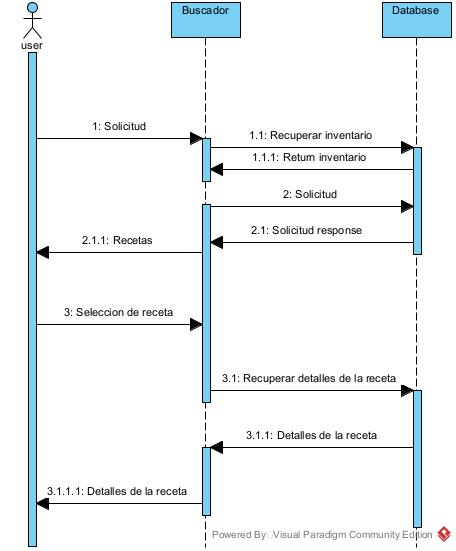
\includegraphics[width=125mm,scale=1]{imagenes/Buscar Receta y ver detalles.jpg}
\caption{Buscar receta y ver detalles}
\label{fig:buscar}
\end{figure}
\begin{figure}[h!]
\centering
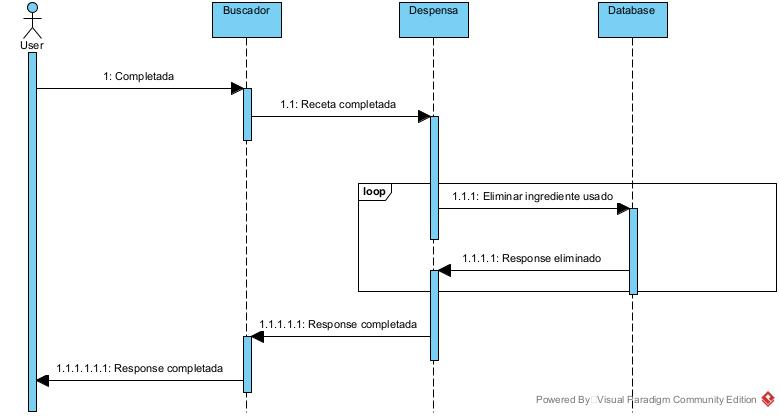
\includegraphics[width=125mm,scale=1]{imagenes/Marcar como completada.jpg}
\caption{Marcar como completada}
\label{fig:completada}
\end{figure}
\begin{figure}[h!]
\centering
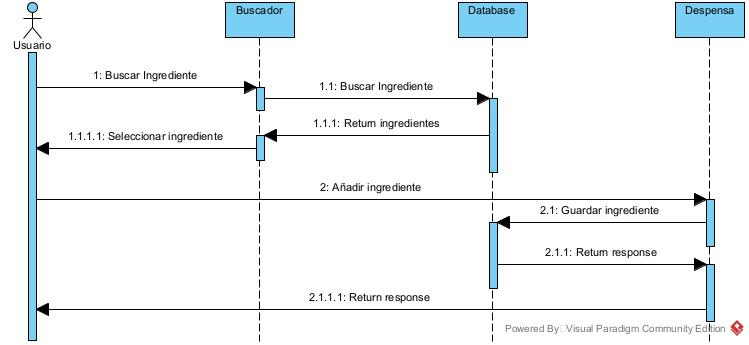
\includegraphics[width=125mm,scale=1]{imagenes/Introducir ingrediente.jpg}
\caption{Añadir ingrediente a la despensa}
\label{fig:addIngrediente}
\end{figure}
\begin{figure}[h!]
\centering
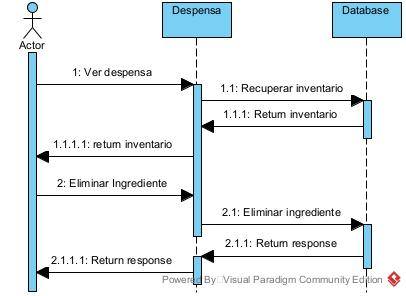
\includegraphics[width=125mm,scale=1]{imagenes/Eliminar ingrediente.jpg}
\caption{Eliminar ingrediente de la despensa}
\label{fig:buscar}
\end{figure}
\begin{figure}[h!]
\centering
\includegraphics[width=125mm,scale=1]{imagenes/Añadir restricciones al buscador.jpg}
\caption{Añadir restricciones al buscador}
\label{fig:aniadir_restricciones}
\end{figure}
\begin{figure}[h!]
\centering
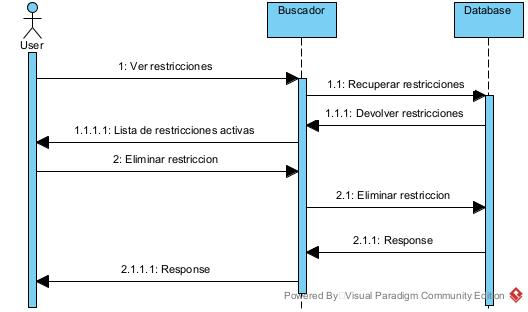
\includegraphics[width=125mm,scale=1]{imagenes/Eliminar restricciones.jpg}
\caption{Eliminar restricciones del buscador}
\label{fig:eliminar_restricciones}
\end{figure}